
\section{Related Works}\label{sec:Related Works}


\subsection{Continual Learning}
Continual learning, also known as lifelong or incremental learning, refers to the ability of a machine learning model to learn from a stream of data over time, while retaining knowledge from previous tasks and adapting to new ones without forgetting~\cite{parisi2019continual}. Unlike traditional learning paradigms, where models are trained on static datasets, continual learning should addresses the dynamic nature of real-world applications, where data distributions and tasks evolve over time.

A central challenge in continual learning is the catastrophic forgetting problem, where a model tends to forget previously learned knowledge when trained on new tasks \cite{french1999catastrophic}. To mitigate this, various strategies have been proposed, including replay-based, regularization-based, and architecture-based methods. For instance, replay-based methods like Experience Replay \cite{rolnick2019experience} store and replay samples from past tasks to maintain performance, while regularization-based methods like Elastic Weight Consolidation (EWC) \cite{kirkpatrick2017overcoming} introduce a regularization term to preserve important parameters for previous tasks. Similarly, Learning without Forgetting (LwF) \cite{li2017learning} uses knowledge distillation to regularize the model by minimizing the divergence between its current and previous outputs. Architecture-based methods allocate distinct subsets of model parameters to different tasks to prevent interference. For example, Progressive Neural Networks (PNNs) \cite{rusu2016progressive} expand the network architecture by adding new layer of parameters for each task while freezing existing ones. In addition Mask-Based Methods \cite{mallya2018piggyback} learns task-specific masks to trigger or suppress parameters dynamically.

In the LLM era, continual pretraining or finetuning has become essential for model iteration and advancement. We focus on continual finetuning, where the most common practice involves replay-based methods, which typically incorporate general corpus to preserve the model's general capabilities for downstream tasks.
In this work, we explore a further integration with regularization-based techniques, i.e., the distillation strategy used in LwF. Specifically, we pre-generate and store the feature representations of the replay samples, which are then used as targets within a distillation framework to effectively leverage this information.
Moreover, we include the LoRA~\cite{hu2022lora} setup since it is widely adopted in finetuning due to its strong generalization and resistance to forgetting. It can be considered as another type of architecture-based method, as it typically trains only a small fraction of parameters.


\begin{figure*}[htbp]
    \centering
    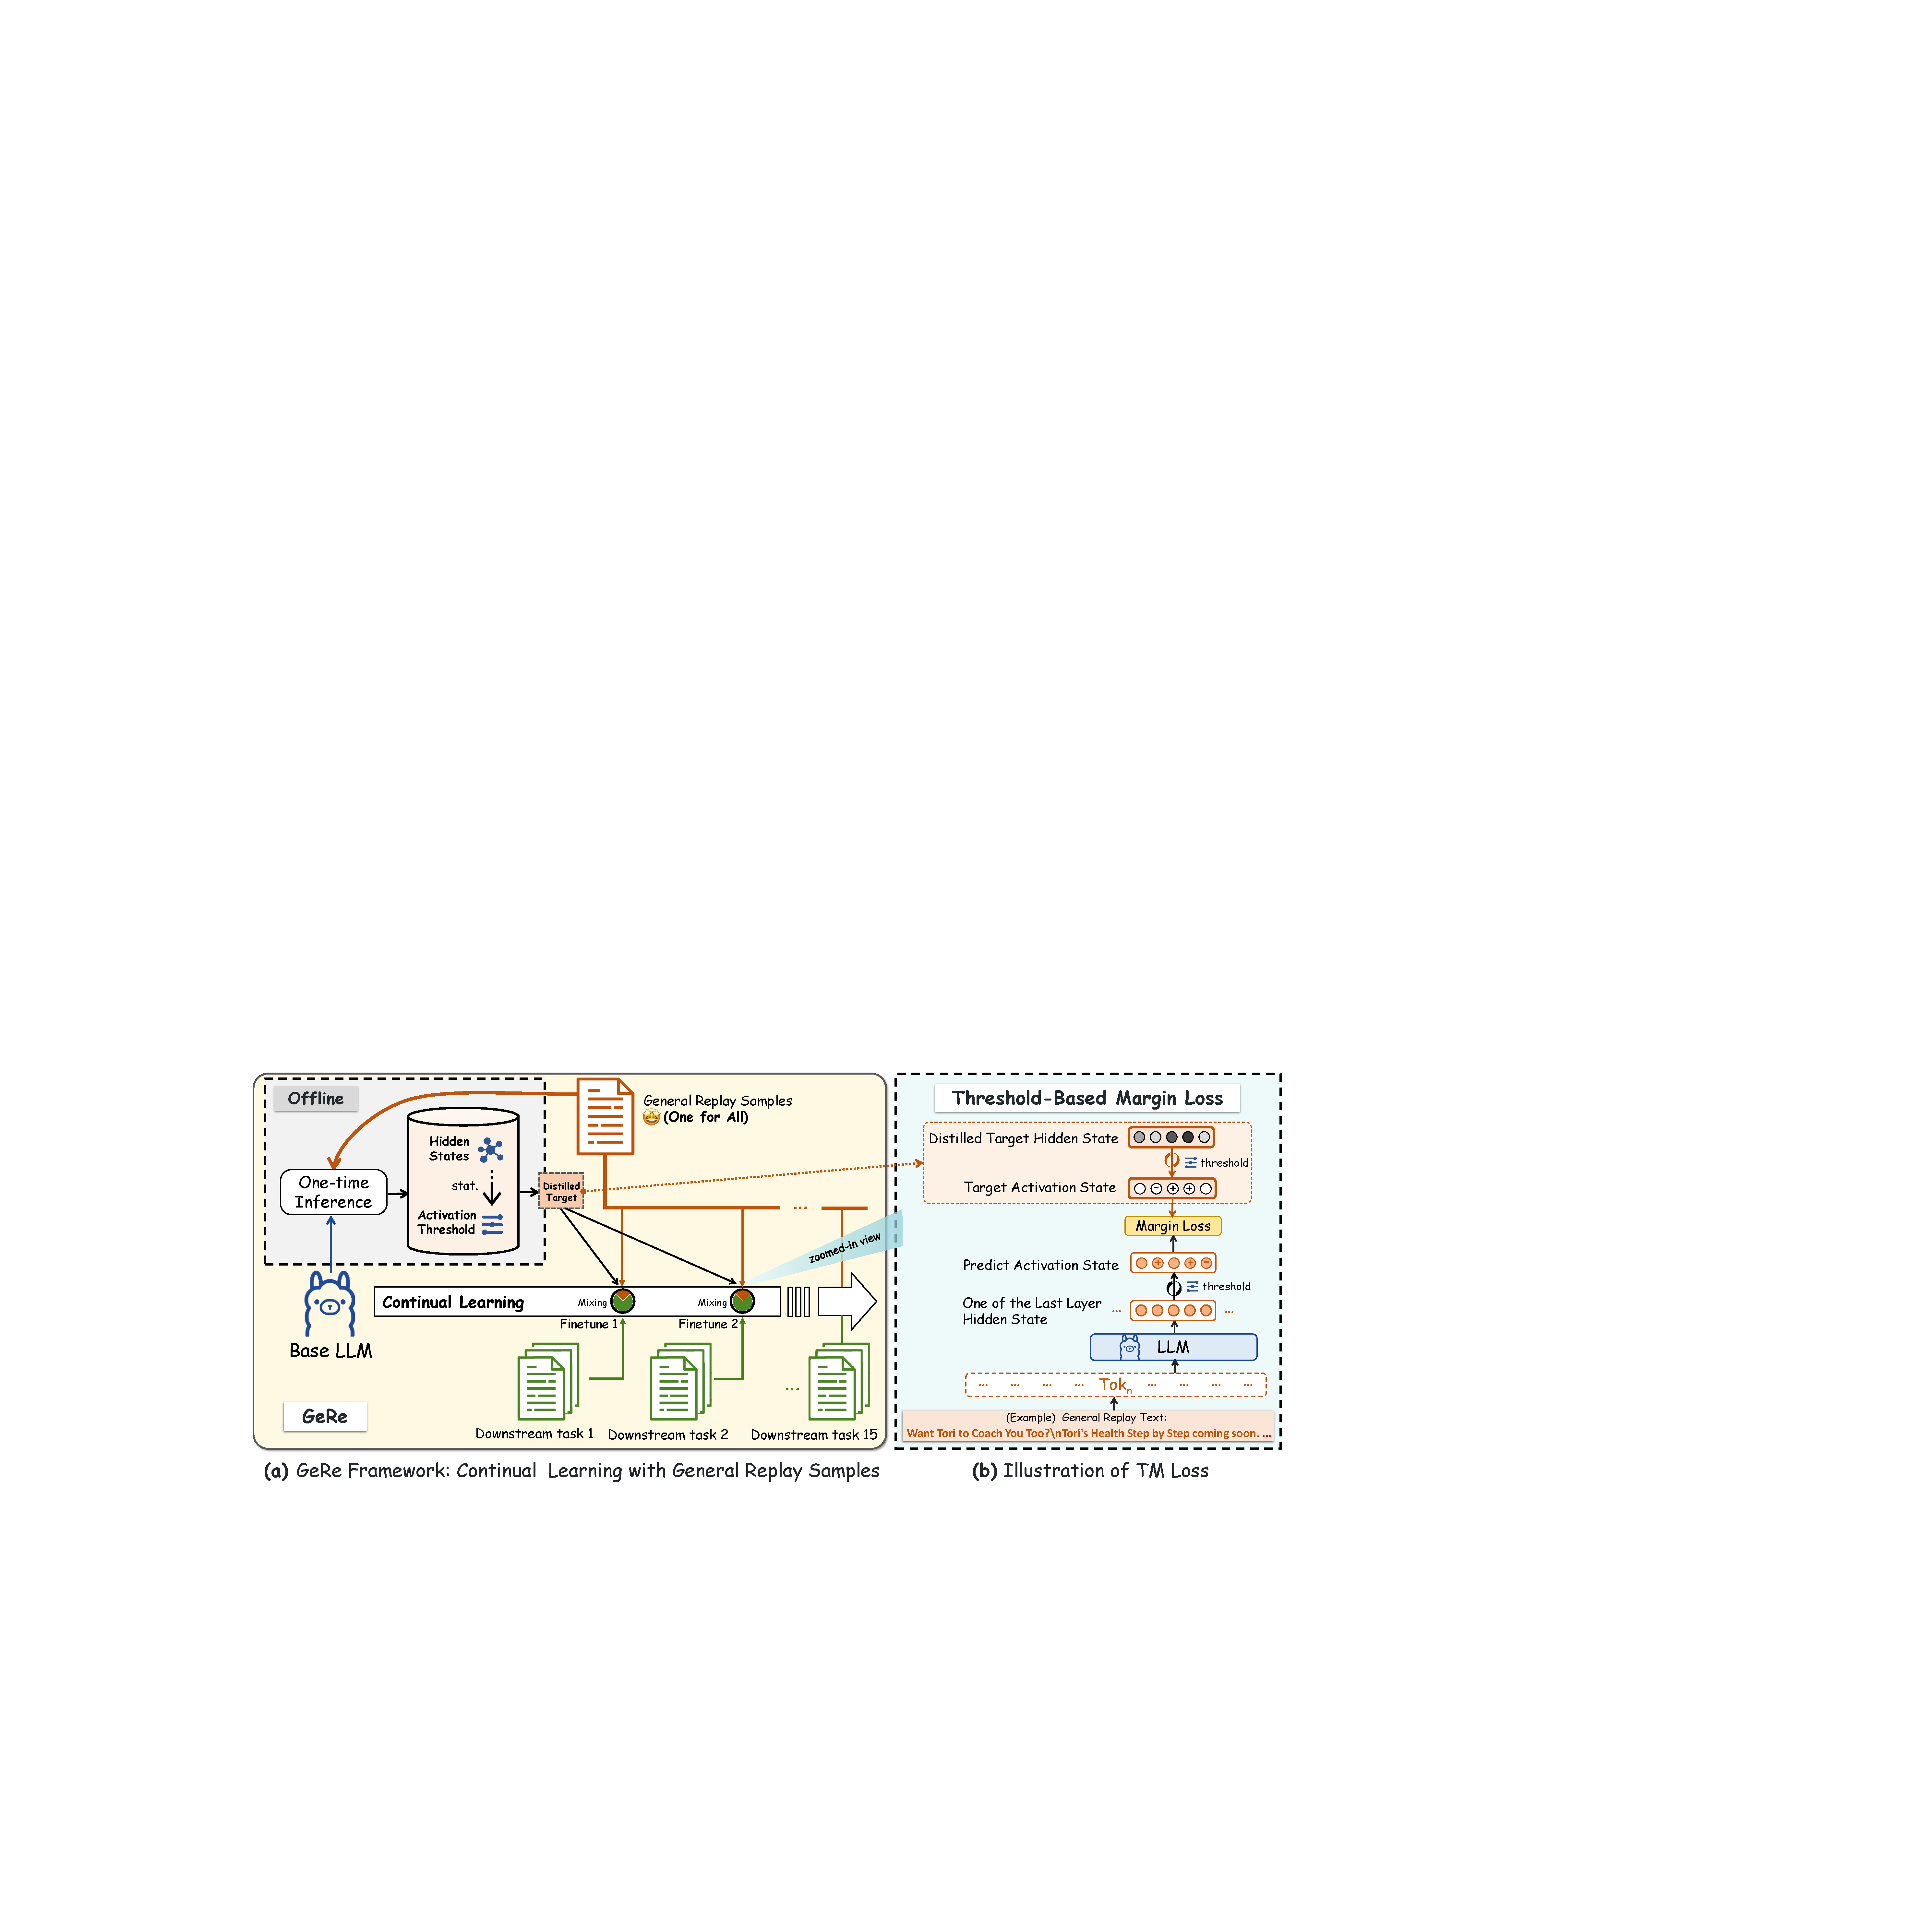
\includegraphics[width=0.9\textwidth]{figtab/main_pic.pdf}
    \caption{(a) Flowchart of the GeRe framework using general replay samples, including distillation of hidden states and the derived activation state in offline mode, and continual learning across sequential tasks with mixing general samples for replay.
    (b) Illustration of threshold-based margin loss, which transforms the hidden values into discrete activation states on both the target and prediction followed by margin loss calculation.
    }
    \label{fig:main_pic}
\end{figure*}

\subsection{Knowledge Distillation}
Knowledge distillation (KD)~\cite{hinton2015distilling} aim to compress large models into smaller, efficient ones by transferring knowledge from a teacher model to a student model. This process is achieved by minimizing the difference between their output distributions, where the student learns from the teacher's soft labels rather than the original dataset's hard labels~\cite{sanh2019distilbert,jiao2020tinybert,zhou2022distilling}.
KD can be implemented generally with two types: logit-based imitation and feature-based imitation~\cite{zhengetal2023ld}. The former involves matching the predictions and target distributions using the Kullback-Leibler divergence (KL) loss with a temperature-based softmax normalization, while the latter focuses on aligning the intermediate representations in the feature space through similarity-based functions. 

KD has already been applied in continual learning, with the key distinction lying in how the target and prediction are defined. Taking LwF for example, when the new task's samples arrived, the model preliminarily computed the logits of these samples at the output heads regarding old tasks, served as the distilled pseudo-targets.
During subsequent training, the real-time predicted logits at these old tasks output heads are constrained to match the precomputed pseudo-targets.
In this case, the teacher and student models are essentially the same model. This self-distillation mechanism~\cite{wang2023distill} enables the model to retain performance on previously learned tasks while adapting to new ones.

However, few research emphasizes similarity of feature in KD typically applied for continual learning of LLMs~\cite{xu2024survey}.
Our work thereby delves deeper into studying efficient mechanism combining replay and distillation methods, where labels or features of replay samples are pre-distilled to serve as pseudo-targets, enabling persistent fitting of replay samples during continual learning.
We empirically compare the effect of using replay samples simply versus leveraging replay samples under both logit-based imitation via KL divergence and feature-based imitation via L1 or L2 function. The study offers a comprehensive comparison of diverse replay strategies.